\chapter{Arquitectura}

\section{Topología de Red}
La red opera en modo IBSS (ad-hoc) sobre Wi-Fi 2.4GHz. Cada nodo escanea el SSID \texttt{AD-HOC-STREAM} al arrancar. Si detecta una celda activa, se une; si no, crea una nueva red y asume el rol de Master.

\section{Roles del Nodo}
\begin{itemize}
    \item \textbf{Master:} Elige canción, inicia servidor ffmpeg UDP multicast, coordina heartbeats.
    \item \textbf{Cliente:} Recibe stream multicast, reproduce con mpv/ffplay, reporta métricas.
\end{itemize}

\section{Visión Holística}
\begin{figure}[h]
\centering
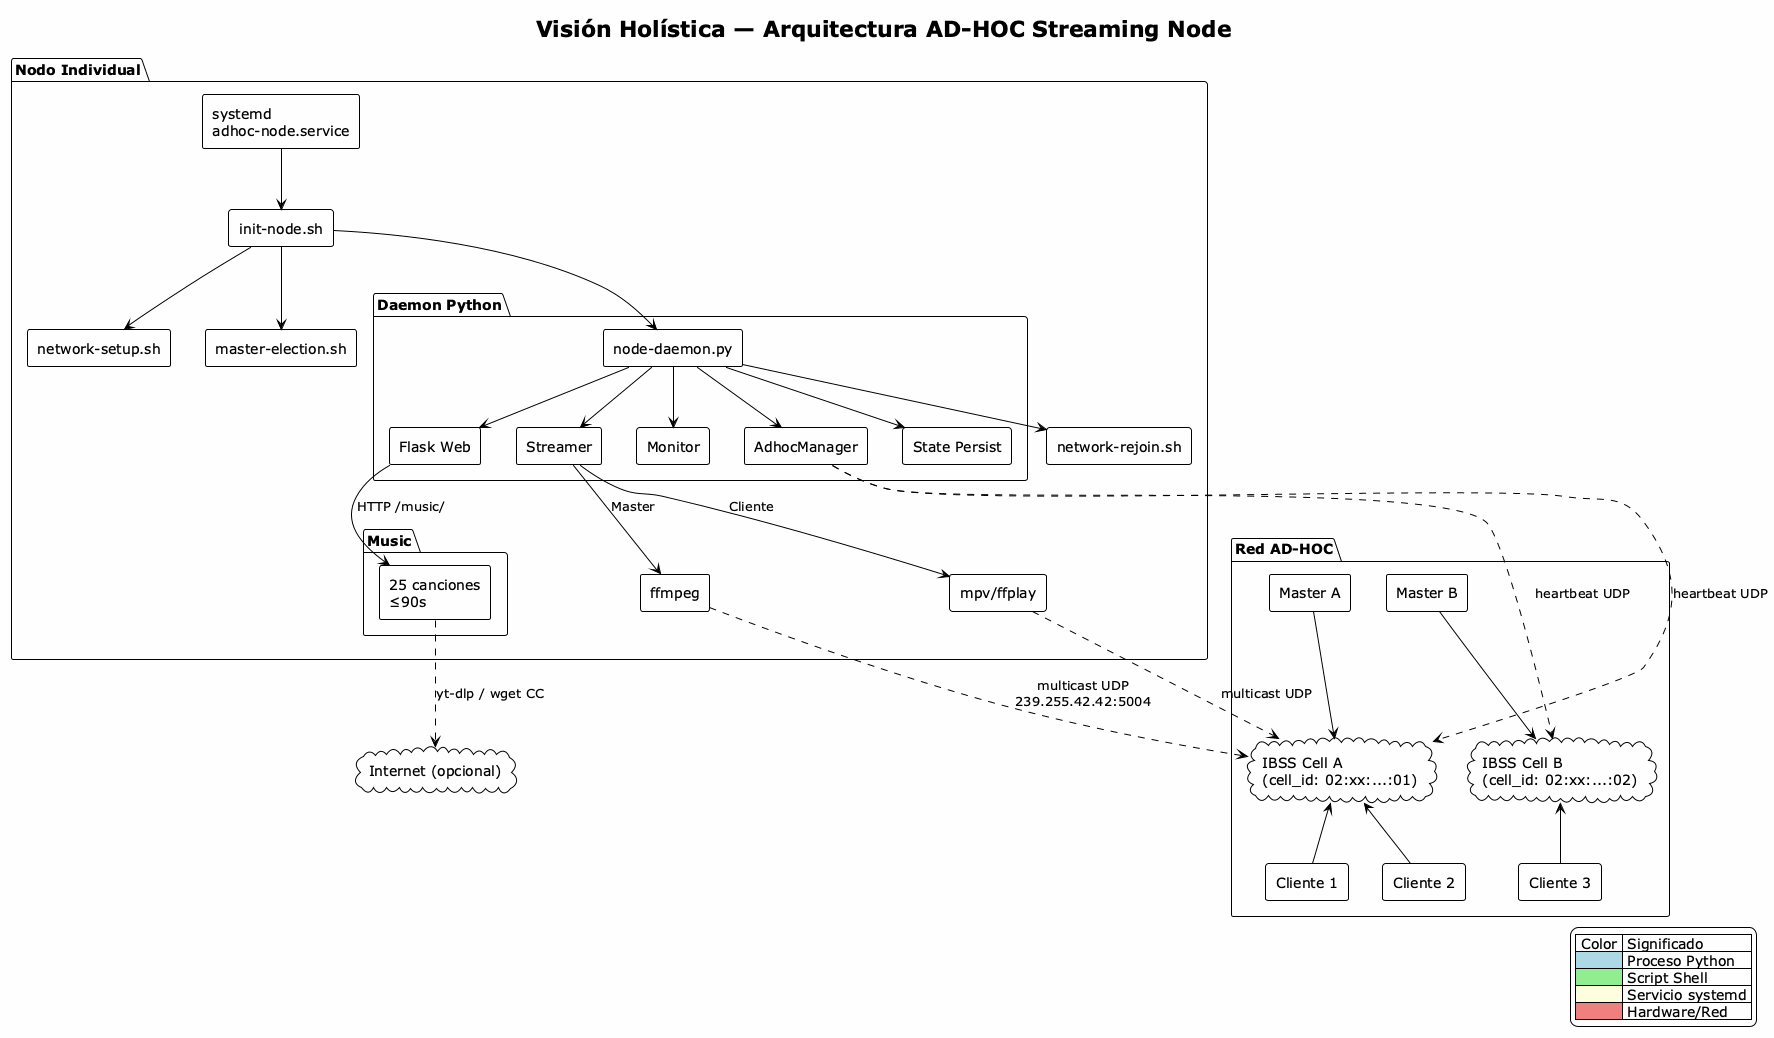
\includegraphics[width=\textwidth]{diagrams/architecture-overview.png}
\caption{Visión holística de la arquitectura AD-HOC Streaming Node.}
\label{fig:overview}
\end{figure}

\section{Topología de Red}
\begin{figure}[h]
\centering
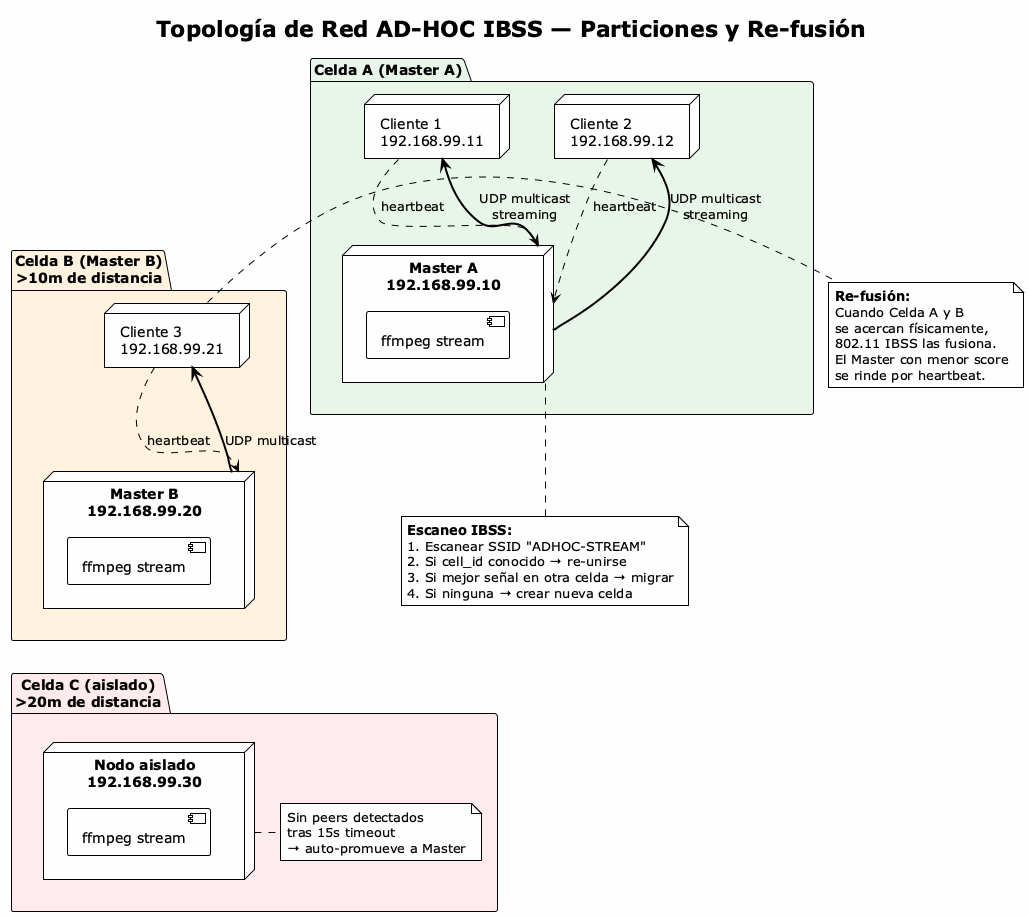
\includegraphics[width=\textwidth]{diagrams/network-topology.png}
\caption{Topología IBSS con celdas dinámicas, particiones y re-fusión.}
\label{fig:topology}
\end{figure}

\section{Diagrama de Despliegue}
\begin{figure}[h]
\centering
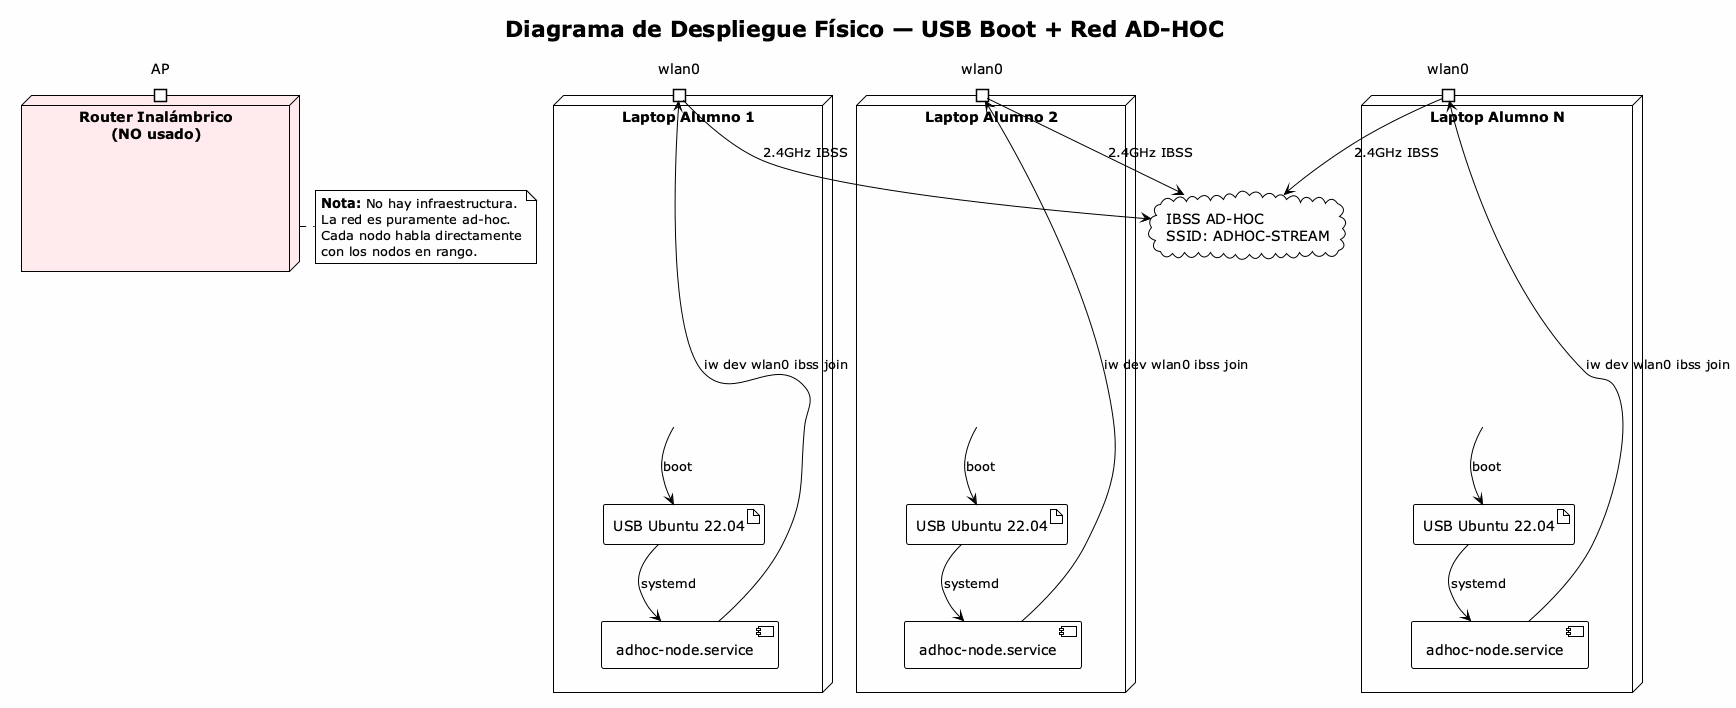
\includegraphics[width=0.8\textwidth]{diagrams/deployment.png}
\caption{Despliegue físico: USB boot en laptops, red ad-hoc sin infraestructura.}
\label{fig:deployment}
\end{figure}

\section{Presupuesto de Enlace}
\begin{figure}[h]
\centering
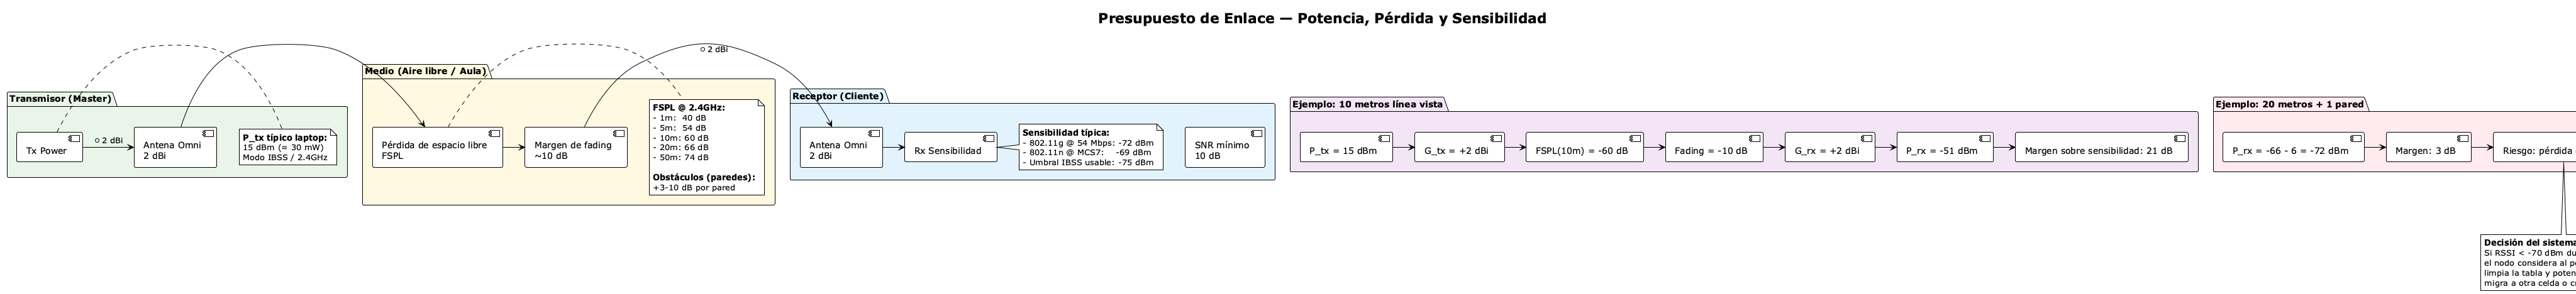
\includegraphics[width=\textwidth]{diagrams/signal-power-link-budget.png}
\caption{Potencia transmitida, pérdida de espacio libre (FSPL) y sensibilidad del receptor.}
\label{fig:linkbudget}
\end{figure}
